\documentclass[10pt,a5paper]{article}
\usepackage[latin5]{inputenc}
\usepackage{amsmath}
\usepackage{amsfonts}
\usepackage{amssymb}
\usepackage{graphicx}
\usepackage{ngerman}
\usepackage[left=1.00cm, right=1.00cm, top=1.00cm, bottom=1.00cm]{geometry}
\author{Christian Böhm}
\usepackage{listings}
\begin{document}
\section{Fachbegriffe}
\begin{tabular}{|c|c|}
\hline IC(integrated circuit) & integriterte schaltkreis \\ 
\hline gate & Gatter \\ 
\hline signal & Signal \\ 
\hline wire,net & Kupferleitung \\ 
\hline CPU(central prozessing unit) & Zentrale Verbarbieutngs einehit \\ 
\hline memory & speicher \\ 
\hline flash memory & Festwertspeicher \\ 
\hline Dram(dynamic random accses memory) & dynamsicher ram \\ 
\hline random acces & wahlfreier zugriff \\ 
\hline ADC(Analog to Digital Converter) & Analgo nach digitalwandler \\ 
\hline DAC(ditial to analog converter) & Digital zu analog Wandler \\ 
\hline OpAmps & Operationsverst�rker \\ 
\hline 0-active(low) & negativ aktiv \\ 
\hline 1-active(high) & positiv aktiv \\ 
\hline keyboard & tastatur \\ 
\hline printer & schreibwerk \\ 
\hline sampling frequency & Abtastfrequenz \\ 
\hline sample & messwert/punkt \\ 
\hline resulution & aufl�sung \\ 
\hline truth/function tabel & wahrheitstabelle \\ 
\hline logical equation & logische Gleichungen \\ 
\hline 
\end{tabular} 
\section{KV Diagramm}4Var
\begin{tabular}{c|c|c|c|c|c}
  & $A$ & $A$ & $\overline{A}$ & $\overline{A}$ &  \\ 
\hline $B$ &  &  &  &  & $D$ \\ 
\hline $B$ &  &  &  &  & $\overline{D}$ \\ 
\hline $\overline{B}$ &  &  &  &  & $\overline{D}$ \\ 
\hline $\overline{B}$ &  &  &  &  & $D$ \\ 
\hline  & $C$ & $\overline{C}$ & $\overline{C}$ & $C$ &  \\ 
\end{tabular} 3 Var
\begin{tabular}{c|c|c|c|c}
  & $A$ & $A$ & $\overline{A}$ & $\overline{A}$ \\ 
\hline $B$ &  &  &  &  \\ 
\hline $\overline{B}$ &  &  &  &  \\ 
\hline  & $C$ & $\overline{C}$ & $\overline{C}$ & $C$ \\ 
 \end{tabular} 2 Var
\begin{tabular}{c|c|c|}
  & $A$ & $\overline{A}$ \\ 
\hline $B$ &  &  \\ 
\hline $\overline{B}$ &  &  \\ 
 \hline
\end{tabular} \vspace{1cm}
\begin{itemize}
\item Konjunktive Normalform: Nullen verkn{"u}pfen
\item Disjunktive Normalform: Einsen verkn{"u}pfen
\end{itemize}
\newpage
\section{Gray-Code}
\begin{itemize}
\item Stetig
\item Hamming Abstand = 1
\item Zahl in Graycode:
\subitem     X1: Dualzahl im Bin�rcode
\subitem X2: Rechts-Shift der Dualzahl um 1 Bit
\subitem X3: Modulo-2-Addition (XOR-Verkn�pfung) von X1 und X2
\subitem X3: gew{"u}nschte Zahl im Graycode.

\end{itemize}
\section{Vollst{"a}ndige Logicksysteme}
\begin{figure}[h]
\centering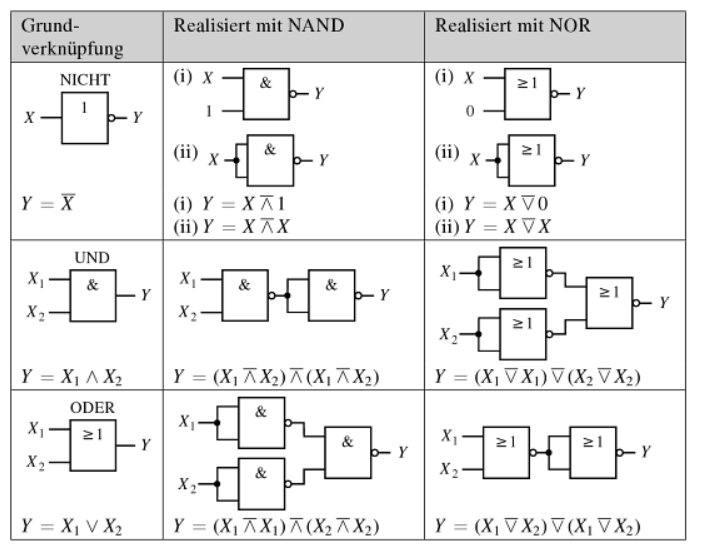
\includegraphics[width=0.7\linewidth]{./nor.png}
\end{figure}


\end{document}